%% BioMed_Central_Tex_Template_v1.06
%%                                      %
%  bmc_article.tex            ver: 1.06 %
%                                       %

%%IMPORTANT: do not delete the first line of this template

%%%%%%%%%%%%%%%%%%%%%%%%%%%%%%%%%%%%%%%%%
%%                                     %%
%%  LaTeX template for BioVis 2014  %%
%%      article submissions     %%
%%          adapted from BMC    %%
%%          <8 Jan 2014>              %%
%% Liz Marai (g.elisabeta.marai@gmail.com) %%
%%                                     %%
%%%%%%%%%%%%%%%%%%%%%%%%%%%%%%%%%%%%%%%%%


%%%%%%%%%%%%%%%%%%%%%%%%%%%%%%%%%%%%%%%%%%%%%%%%%%%%%%%%%%%%%%%%%%%%%
%%                                                                 %%
%%%%%%%%%%%%%%%%%%%%%%%%%%%%%%%%%%%%%%%%%%%%%%%%%%%%%%%%%%%%%%%%%%%%%

%%% additional documentclass options:
%  [doublespacing]
%  [linenumbers]   - put the line numbers on margins

%%% loading packages, author definitions

\documentclass[twocolumn]{bmcart}% uncomment this for twocolumn layout 



%%% Load packages
%\usepackage{amsthm,amsmath}
%\RequirePackage{natbib}
%\RequirePackage{hyperref}
\usepackage[utf8]{inputenc} %unicode support
%\usepackage[applemac]{inputenc} %applemac support if unicode package fails
%\usepackage[latin1]{inputenc} %UNIX support if unicode package fails
\usepackage{graphicx}

%%%%%%%%%%%%%%%%%%%%%%%%%%%%%%%%%%%%%%%%%%%%%%%%%
%%                                             %%
%%  If you wish to display your graphics for   %%
%%  your own use using includegraphic or       %%
%%  includegraphics, then comment out the      %%
%%  following two lines of code.               %%
%%%%%%%%%%%%%%%%%%%%%%%%%%%%%%%%%%%%%%%%%%%%%%%%%


%\def\includegraphic{}
%\def\includegraphics{}



%%% Put your definitions there:
\startlocaldefs
\endlocaldefs


%%% Begin ...
\begin{document}

%%% Start of article front matter
\begin{frontmatter}

\begin{fmbox}
\dochead{Research}

%%%%%%%%%%%%%%%%%%%%%%%%%%%%%%%%%%%%%%%%%%%%%%
%%                                          %%
%% Enter the title of your article here     %%
%%                                          %%
%%%%%%%%%%%%%%%%%%%%%%%%%%%%%%%%%%%%%%%%%%%%%%

\title{SketchBio: A Scientist's 3D Interface for Molecular Modeling and Animation}

%%%%%%%%%%%%%%%%%%%%%%%%%%%%%%%%%%%%%%%%%%%%%%
%%                                          %%
%% Do not enter the authors here for        %%
%%  a double-blind review. Otherwise        %%
%% specify information, if available,       %%
%% in the form:                             %%
%%   <key>={<id1>,<id2>}                    %%
%%   <key>=                                 %%
%% Comment or delete the keys which are     %%
%% not used. Repeat \author command as much %%
%% as required.                             %%
%%                                          %%
%%%%%%%%%%%%%%%%%%%%%%%%%%%%%%%%%%%%%%%%%%%%%%
\author[
     addressref={aff1},
  % noteref={n2},
   email={swaldon@cs.unc.edu}
]{\inits{SW}\fnm{Shawn} \snm{Waldon}}
\author[
   addressref={aff1},                   % id's of addresses, e.g. {aff1,aff2}
   %corref={aff1},                       % id of corresponding address, if any
   %noteref={n1},                        % id's of article notes, if any
  email={taylorr@cs.unc.edu}   % email address
]{\inits{RT}\fnm{Russell} \snm{Taylor} \suffix{II}}
\author[
	addressref={aff1},
	email={pthomps@live.unc.edu}
]{\inits{PT}\fnm{Peter} \snm{Thompson}}

%%%%%%%%%%%%%%%%%%%%%%%%%%%%%%%%%%%%%%%%%%%%%%
%%                                          %%
%% Enter the authors' addresses here        %%
%%                                          %%
%% Repeat \address commands as much as      %%
%% required.                                %%
%%                                          %%
%%%%%%%%%%%%%%%%%%%%%%%%%%%%%%%%%%%%%%%%%%%%%%

\address[id=aff1]{%                           % unique id
  \orgname{University of North Carolina at Chapel Hill}, % university, etc
  \postcode{27599}                                % post or zip code
  \city{Chapel Hill, NC},                              % city
  \cny{US}                                    % country
}
%\address[id=aff2]{%                           % unique id
%  \orgname{Anonymous Also}, % university, etc
%  \street{210 South Bouquet},                     %
%  \postcode{15260}                                % post or zip code
%  \city{Williamsburg},                              % city
%  \cny{UK}                                    % country
%}


%%%%%%%%%%%%%%%%%%%%%%%%%%%%%%%%%%%%%%%%%%%%%%
%%                                          %%
%% Enter short notes here                   %%
%%                                          %%
%% Short notes will be after addresses      %%
%% on first page.                           %%
%%                                          %%
%%%%%%%%%%%%%%%%%%%%%%%%%%%%%%%%%%%%%%%%%%%%%%

\begin{artnotes}
%\note{Sample of title note}     % note to the article
%\note[id=n1]{Equal contributor} % note, connected to author
%\note[id=n2]{Equal contributor} % note, connected to author
%\note[id=n3]{Equal contributor} % note, connected to author
%\note[id=n4]{Project leader and equal contributor} % note, connected to author
\end{artnotes}

\end{fmbox}% comment this for two column layout

%%%%%%%%%%%%%%%%%%%%%%%%%%%%%%%%%%%%%%%%%%%%%%
%%                                          %%
%% The Abstract begins here                 %%
%%                                          %%
%% Please refer to the Instructions for     %%
%% authors on http://www.biomedcentral.com  %%
%% and include the section headings         %%
%% accordingly for your article type.       %%
%%                                          %%
%%%%%%%%%%%%%%%%%%%%%%%%%%%%%%%%%%%%%%%%%%%%%%

\begin{abstractbox}

\begin{abstract} % abstract, must be under 350 words
%\parttitle{First part title} %if any
%Text for this section.

\parttitle{Background} Lorem ipsum dolor sit amet, consectetuer adipiscing elit, sed diam nonummy nibh euismod tincidunt ut laoreet dolore magna aliquam erat volutpat. Ut wisi enim ad minim veniam, quis nostrud exerci tation ullamcorper suscipit lobortis nisl ut aliquip ex ea commodo consequat. 

\parttitle{Results} We introduce a system for lorem ipsum dolor sit amet, consectetuer adipiscing elit, sed diam nonummy nibh euismod tincidunt ut laoreet dolore magna aliquam erat volutpat. Ut wisi enim ad minim veniam, quis nostrud exerci tation ullamcorper suscipit lobortis nisl ut aliquip ex ea commodo consequat. 

\parttitle{Conclusions}  Lorem ipsum dolor sit amet, consectetuer adipiscing elit, sed diam nonummy nibh euismod tincidunt ut laoreet dolore magna aliquam erat volutpat. Ut wisi enim ad minim veniam, quis nostrud exerci tation ullamcorper suscipit lobortis nisl ut aliquip ex ea commodo consequat. Duis autem vel eum iriure dolor.


%\parttitle{Second part title} %if any
%Text for this section.
\end{abstract}

%%%%%%%%%%%%%%%%%%%%%%%%%%%%%%%%%%%%%%%%%%%%%%
%%                                          %%
%% The keywords begin here                  %%
%%                                          %%
%% Put each keyword in separate \kwd{}.     %%
%%                                          %%
%%%%%%%%%%%%%%%%%%%%%%%%%%%%%%%%%%%%%%%%%%%%%%

\begin{keyword}
\kwd{Molecular Modelling}
\kwd{Animation}
\kwd{Collision Detection}
\end{keyword}

% MSC classifications codes, if any
%\begin{keyword}[class=AMS]
%\kwd[Primary ]{}
%\kwd{}
%\kwd[; secondary ]{}
%\end{keyword}

\end{abstractbox}
%
%\end{fmbox}% uncomment this for twcolumn layout

\end{frontmatter}

%%%%%%%%%%%%%%%%%%%%%%%%%%%%%%%%%%%%%%%%%%%%%%
%%                                          %%
%% The Main Body begins here                %%
%%                                          %%
%% Please refer to the instructions for     %%
%% authors on:                              %%
%% http://www.biomedcentral.com/info/authors%%
%% and include the section headings         %%
%% accordingly for your article type.       %%
%%                                          %%
%% See the Results and Discussion section   %%
%% for details on how to create sub-sections%%
%%                                          %%
%% use \cite{...} to cite references        %%
%%  \cite{koon} and                         %%
%%  \cite{oreg,khar,zvai,xjon,schn,pond}    %%
%%  \nocite{smith,marg,hunn,advi,koha,mouse}%%
%%                                          %%
%%%%%%%%%%%%%%%%%%%%%%%%%%%%%%%%%%%%%%%%%%%%%%

%%%%%%%%%%%%%%%%%%%%%%%%% start of article main body
% <put your article body there>


%%%%%%%%%%%%%%%%
%% Background %%
%%
\section*{Background}

We found ourselves repeatedly using 2D hand-drawings of complex 3D structures and their interactions in discussions with our close collaborators in cell biology, pathology, and chemistry, despite the fact that the 3D crystal structures of the proteins making up these structures were known.  Hanging David Goodsell's excellent ``Molecular Machinery" poster \cite{Goodsell} showing renderings of many of these molecules and their interactions helped to grow our shared understanding of the structures in the mitotic spindle, but real progress was made when we hired an artist to draw 3D scale models of the structures each week and then develop 3D computer models \cite{taylor2012}.

Our group is not alone.  Discussions among collaborators are often done using 2D whiteboard sketches.  Presentations often consist of pasted images and 2D Powerpoint animations.

Because of the difficulties involved in learning and using 3D modeling and rendering software, many scientists hire professional computer programmers and/or animators to work with them to create models and animations rather than use these programs themselves.  This indirection both slows the discovery process and provides opportunities for miscommunication. As toolsmiths, our aim is to provide scientists with a tool that is so rapid to learn and use that they can create these models and animations themselves.

This paper describes that tool, SketchBio.

\subsection*{Driving Problems}
Fred Brooks points out that the best way to construct a tool that is generally usable is to focus on several very different specific problems and build a tool that solves them.  We are following this approach.

The first driving problem for this project is collaborator Susan Lord's desire to construct a protofibril model based on geometric constraints among a set of fibrinogen monomers.  Based on the crystallized structures of fibrin monomers from different species and on only two sets of known interactions \cite{lord2007fibrinogen}, she sought to construct 3D protofibril structures matching those seen in TEM studies.  Over the process of several months, she and her students worked with Resource staff scientist Joe Hsiao to use the powerful UCSF Chimera tool to construct such a model \cite{lordSubmitted}.  Building this model required repeated iteration of hand-placement of two molecules (using multiple 2D mouse interactions), followed by using replication tools to develop candidate models, which were then evaluated against the data.  Lord's desired use of SketchBio was to construct this protofibril rapidly and semi-automatically by specifying which location on each fibrin should be in close contact with other molecules and by specifying that the molecules do not overlap.  This same capability will enable generation of other self-symmetric structures such as actin filaments and microtubules.

Our second driving problem is comes from Peter Thompson in Sharon Campbell's lab.  Peter wants to construct 3D models and animations of the interaction between actin filaments and vinculin.  He has used SketchBio to reproduce 3D geometry from example structures found in the literature and to generate animated videos to show his hypothetical interactions to colleagues.  He is particularly interested in using SketchBio as a thinking tool to determine how mutations in the vinculin can turn the normally-straight actin filaments into helices.  The resulting optimization algorithms will enable other scientists to semi-automatically construct multi-protein structures that match TEM images.

The third driving problem comes from our collaboration with Kerry Bloom, described above.  As in the Lord case, each step of model generation has required support from an artist, animator, and/or programmer to convert Bloom's concepts and those of his students into geometry for rendering and simulation.  Our program-generated models exhibit more symmetry than the experimental results only because of the difficulty in specifying more complex models that meet the geometric constraints (cohesin loops surrounding four chromatin, no self-intersection or entanglement, etc.).  Bloom needs SketchBio to support (i) the rapid generation of long coarse-grained interacting polymer chains and their connection to coarse-grained models of symmetric microtubules, (ii) the construction of linked but non-colliding protein-chromosome structures, and (iii) production of simulated fluorescence images from the resulting structures.

Our final drivign problem also comes from this same collaboration.  Many proteins beyond cohesin and condensin contribute to mitosis, and Kerry Bloom is interested in them all.  His lab is able to fluorescently label both these proteins and chromosome locations, and use multi-color or FRET techniques to determine relative distances and orientations between pairs of proteins.  With accurate localization and tracking for 3D images, these techniques provide partial information on the 3D layout of proteins and chromosomes in wild-type and mutant mitotic spindles.  Building matching models requires the development of mass-spring-driven semi-automatic layout of proteins.  This will provide a partial set of constraints for the scientist to construct protein-protein and protein-chromosome complexes that match experimental data.  With these enhancements, SketchBio will be widely useful to other researchers for the generation of hypothetical protein-complex structures from partial data.

\subsection*{Prior Work}
\paragraph*{Related Applications:}

Subcellular macromolecular modelling for animation is usually done with programs that are difficult to learn, and which are controlled by keyboard and a 2D mouse.

Several other applications target similar goals including UCSF Chimera \cite{pettersen2004ucsf}, the Molecular Control Toolkit \cite{sabirmolecular} and PresentaBALL \cite{nickelspresentaball}.  While Chimera has many features that can be useful to scientists, its complex nature makes it difficult to learn, and the mouse and keyboard controls it supports are not optimal for manipulating objects in three dimensions.  The Molecular Control Toolkit is also aimed at molecular modeling, providing an additional user interface for existing tools using gestures to control motions of objects with a Kinect or Leap Motion device \cite{sabirmolecular}.  However, mapping separate inputs to different degrees of freedom for manipulation usually decreases the user's performance\cite{bowman20043d} and the Molecular Control Toolkit maps a separate gesture to each degree of freedom.  Another tool aimed at simplifying the creation of molecular animations, PresentaBALL uses an interactive web interface to an existing molecular modeling tool \cite{nickelspresentaball}.  This allows widespread use but does nothing to assist in the difficult problem of placing things in 6 degrees of freedom.

% we aren't really talking about the simplification here... leaving this paragraph out for now
%A common bottleneck in interactive modeling and animation applications is the speed of rendering a complex scene.  A key technique in improving the rendering speed of an application is reducing the complexity of the objects that are drawn.  This is done by replacing objects with imposters which are simpler pieces of geometry that result in the same or a very similar result being rendered.  Imposters can be difficult to notice, especially if they are far from the camera and the resulting screen area is small.  One type of imposter is a simplified version of the geometry that is textured to look like the more complex version \cite{decoret2003billboard}\cite{erikson1998simplification}\cite{cohen1998appearance}.  Another common imposter is a square that has a pre-rendered image of the more complex object as its texture.  As long as the viewpoint stays near the same position the discrepancies between this and the actual geometry will be small \cite{aliaga1996visualization}\cite{maciel1995visual}.  The level of simplification of an object can also be dynamically determined according to the amount of the allotted rendering time that is needed to draw each level of detail [XXX cite vtkLODActor.  How?].

\paragraph*{Collision Detection:}
In order to create a model or animation that is useful, collisions between molecules must be detected and handled or reported to the user.  If there are $n$ molecules in the scene, then each of the $n\choose 2$ pairs of molecules must be tested for collisions.  Between each pair of molecules tested, each single unit in one must be tested against each single unit in the other.  This means that collision detection has a complexity of $\mathcal{O}(n^2)$ in the number of primitives since there can be $\mathcal{O}(n^2)$ collisions if everything is colliding with everything else.  However, in more realistic examples, there will typically be far fewer collisions than potential collisions and so optimizations can be done on the search to reduce the expected complexity.  The best expected complexity uses sweep and prune methods and assumes the primitives are sorted in some dimension to get a complexity of $\mathcal{O}(n + c)$ where c is the number of colliding pairs \cite{tracy2009efficient}.  Described in Tracy, Buss \& Woods is a complex method of keeping the list of primitives sorted in some dimension to avoid the $\mathcal{O}(n lg(n))$ cost of sorting the list at each timestep as objects move \cite{tracy2009efficient}.  A somewhat simpler approach is to use a space partitioning method to rule out tests that do not need to be performed.  Space partitioning can be done using a tree of primitives and the volumes that bound them, called a bounding volume hierarchy.  This approach is used by libraries such as the PQP library created by the UNC GAMMA group \cite{PQP}.  An alternate kind of space partitioning is to divide space into “bins” and group the objects by which bin they are in.  Then only the other primitives in the same bin or very nearby bins need to be tested against them.  This type of algorithm is especially effective on GPUs where many local groups may be run in parallel \cite{oat2008efficient}.

\paragraph*{Background Processes: }
As more and more computers move to multicore processors, applications can take advantage of the background CPUs to do work that is not immediately necessary.  This can include calls to other applications in the background to precompute results or even to create images to be rendered.  A system for seamless integration of applications for visualization was done by Rungta et. al by adding a layer above all of the applications of interest to pass events back and forth \cite{rungta2013manyvis}.

\paragraph*{SketchBio:}
This work presents SketchBio, a tool for creating models and animations of proteins and other macromolecular structures.  In order to promote usability, SketchBio is designed to run on a laptop such as a scientist would have and use inexpensive commercial hardware.  The hardware of choice is the Razer Hydra, a pair of six degree of freedom trackers with buttons and high-hats.

\section*{Methods}

SketchBio is a system for understanding subcellular biology through the building of complex 3D macromolecular structures, and animating the structures over time.   The modeling, and rendering of these hypothetical situations currently involves accessing and using a number of tools and databases (PDB, UCSF Chimera, Blender, and MicroscopeSimulator) and then converting files and data to pass between tools.  It also involves manual placement of 3D objects, which is currently done using clunky 2D input devices and by-eye detection and avoidance of collisions.  Some scientists hire professional computer programmers or animators to create 3D models and animations for them due to the high learning curve of typical modeling and animations, adding an additional communication barrier to the process.  As a result, it often takes a team months to produce an acceptable model or animation.  We aim to reduce this to a single person working for hours or days.

\subsection*{Design Decisions}
A key goal of SketchBio is to be an application that a scientist can run in their current computers.  This eliminates the possibility of stereo displays and associated graphics cards and haptic feedback devices as these devices are prohibitively expensive and scientists will not purchase them for the purpose of running a single application.  Therefore SketchBio uses the Razer Hydra input device which has a pair of 6 degree-of-freedom trackers, one for each hand with a high-hat and several buttons on each tracker.  XXX - paragraph seem incomplete

Scientists are not likely to adopt a tool that requires them to spend a lot of time working on the computer for little payout.  SketchBio aims to minimize and consolidate the time that the scientist spends in front of the computer by running many jobs in the background.  Almost all systems in use in labs have multiple processors and in many cases the background processors can be utilized without interfering with other applications.  SketchBio takes advantage of this in two ways: using background threads to do non-immediate work and calling subprocesses to perform tasks that are already implemented externally.  This allows the scientist to avoid waiting on non-essential background output--to continue working and to perform long-running operations in the background while they work on other things.

% XXX I'm not sure about this paragraph - half of it is new but I combined it with an exisiting paragraph when redoing the sections
The design of SketchBio avoids reimplementing existing features where possible, instead using python scripting to control subprocesses to perform these operations.  When reading in PDB files, instead of writing a PDB file reader, SketchBio calls UCSF Chimera as a subprocess to read in the protein and create a displayable surface from it.  Instead of writing a new rendering library, SketchBio uses the python scripting interface of Blender to create a Blender project that will produce the desired animation.  SketchBio uses the open source Qt and VTK\cite{VTKbook} libraries for its user interface and internal rendering and the open source Proximity Query Package (PQP) for collision detection \cite{PQP}.  The VRPN library is used to communicate with the Razer Hydra input device \cite{taylor2001vrpn}.

\subsection*{System Overview}

\begin{figure}[t]
\centering
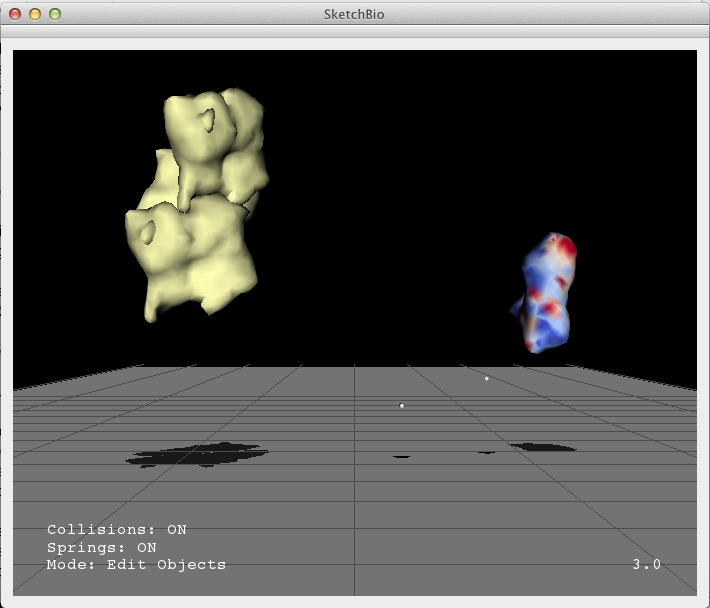
\includegraphics[width=0.8\columnwidth]{actinVinculin.png}
\caption{A screen shot from SketchBio showing three actin monomers on the left colored yellow and the tail region of the vinculin protein on the right colored by surface charge.}
\label{fig:actin_vinculin}
\end{figure}

Figure \ref{fig:actin_vinculin} shows a screenshot of the SketchBio user interface with three actin molecules (left) and the tail region of a vinculin molecule (right).  The small white spheres in the center represent the two tracked hand-held controllers.  In the lower left, status information about the current state of the system can be seen.  One of the main uses of SketchBio is creating animations, this project is an animation and the time in the animation is seen on the lower right in seconds.  This image also shows SketchBio coloring the objects, both solid colors like the yellow actin and according to some dataset like the vinculin tail on the right that is colored by surface charge.

\paragraph*{Importing Molecules:}
SketchBio generates the molecular surfaces using UCSF Chimera.  This subprocess is controlled via python scripting and a plugin was written for Chimera's python interface in order to export data from Chimera in the VTK file format.  This data includes not only the surface geometry but other data sets as well such as residue and chain identifier that map to a specific location on the surface and electrostatic potential on the surface.  These datasets allow the objects to be colored similar to the vinculin tail on the right.

\begin{figure}[h]
\centering
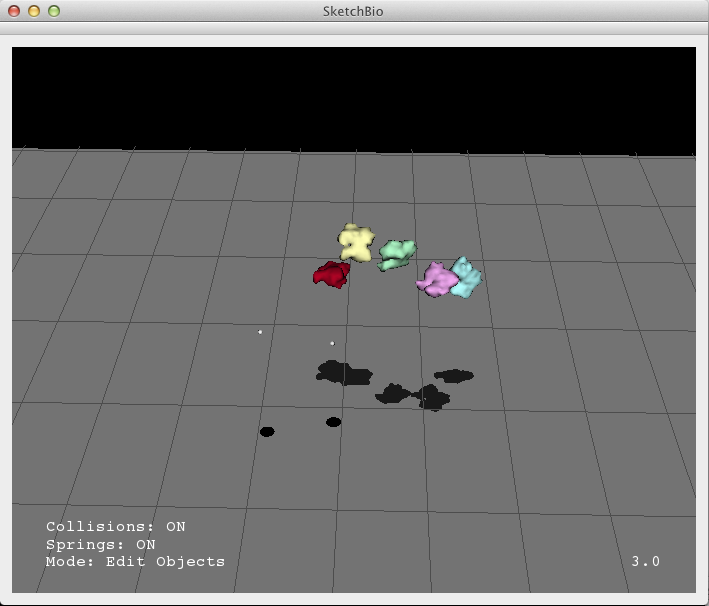
\includegraphics[width=0.8\columnwidth]{shadow_plane.png}
\caption{A screenshot from SketchBio showing colored molecules and a different camera angle to emphasize the shadow plane's effect.}
\label{fig:shadow_plane}
\end{figure}

\paragraph*{Shadows:}
Selection in SketchBio involves moving the tracker to a location within the bounding box of the object, determining the relative depth between the tracker and the object is an important and often-performed task.  To provide additional depth cues, SketchBio displays a ground plane that is always rendered below the viewpoint no matter the direction or position of the viewpoint and projects the "shadows" of objects onto this plane.  The trackers also cast shadows onto this plane and these are darker to easily distinguish between the two.  Hendrix and Barfield found the most effective techniques for aiding in depth estimation are a textured plane and lines dropped from the center of an object to the textured plane \cite{Hendrix1995103}.  SketchBio assumes a light infinitely far away in the default camera's up direction which gives the same absolute position against the textured surface as the drop-lines while also giving information about how close the boundaries of two objects are to each other.  The user can also rotate the camera while leaving the light and shadow plane fixed to get a better understanding of the scene through motion parallax [See Figure \ref{fig:shadow_plane}].

\begin{figure}[h]
\centering
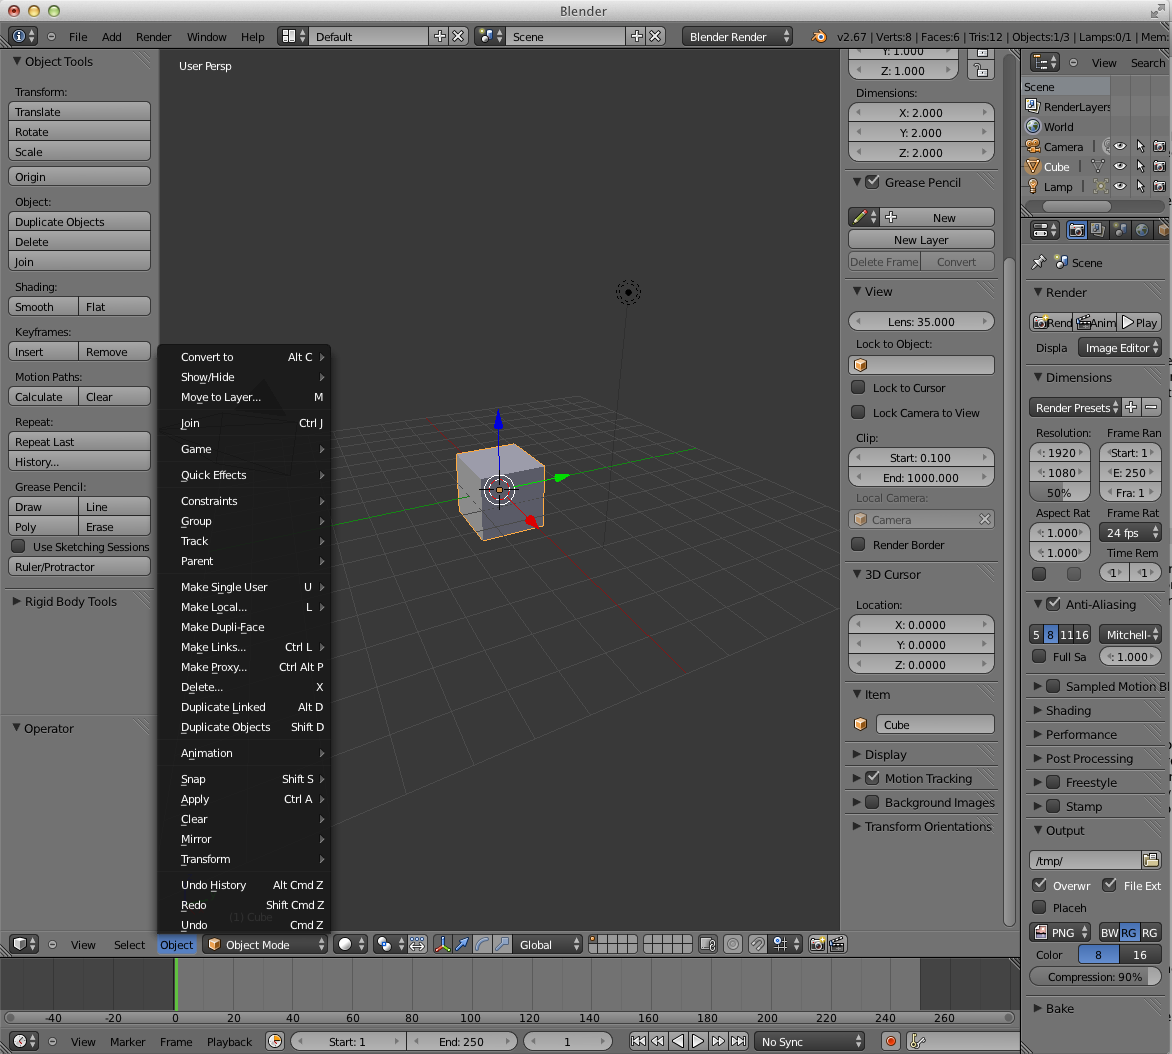
\includegraphics[width=0.8\columnwidth]{blender_interface.png}
\caption{A screenshot showing the complexity of Blender's user interface.}
\label{fig:blender_interface}
\end{figure}

\paragraph*{Animations:}
For scientists creating animations of molecules, SketchBio provides a basic interface to a much more complex system.  Blender is a production level animation and rendering tool.  It has an extremely complex user interface with dozens of hotkeys, menus and buttons (see Figure \ref{fig:blender_interface}.  Blender also has a python scripting interface that allows access to all of its functionality.  SketchBio uses Blender's python scripting interface to create its animations and render them in a high quality rendering engine, but provides a much simpler way to access that interface.  However, Blender is a complex tool that takes weeks or months to learn to use well.  SketchBio provides simple operations, moving along the video timeline and setting keyframes on objects.  Keyframes save not only position and orientation of the objects but also other changeable aspects such as color.  These values are then interpolated between the keyframes to produce the motion in the animation.  These values are also exported to Blender with a set of global settings for effects and position of light sources to produce a full quality rendering.

\begin{figure}[h]
\centering
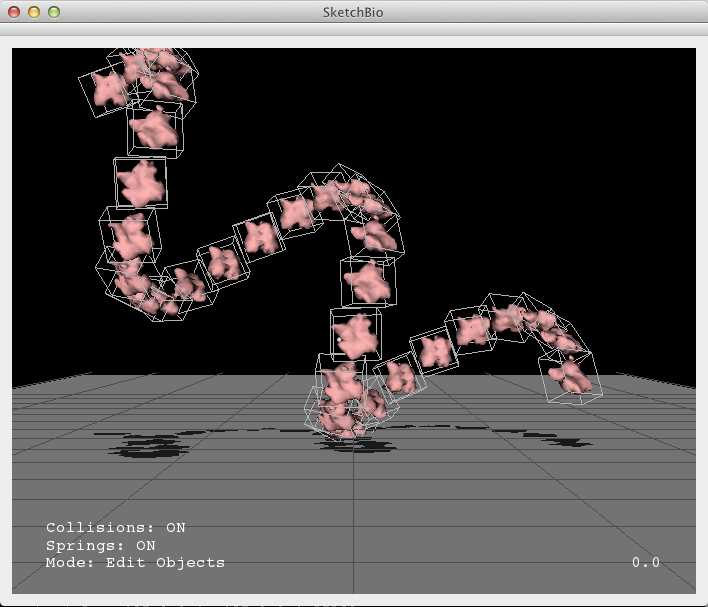
\includegraphics[width=0.8\columnwidth]{crystalByExample.png}
\caption{A screenshot from SketchBio showing a contrived crystal-by-example structure that forms a helix.}
\label{fig:crystal_by_example}
\end{figure}
\paragraph*{Crystal-by-example:}
SketchBio has some features that allow quick creation of typical biological structures.  Repeated structures that are formed from a single type of protein such as the contrived example in figure \ref{fig:crystal_by_example} are somewhat common in biology, so the ‘crystal-by-example' feature was added.  This feature allows example molecules A and B to define the entire repeated structure.  Given $T_A$ and $T_B$, the transformation matrices that define the positions of A and B relative to the world origin, the transformation from A's coordinate system to B's coordinate system, $T_{AB} = T_A^-1*T_B$, can be computed.  Then B's position can be rewritten $T_B = T_A*T_{AB}$.  This allows the creation of the next repeated molecule, C, with position $T_C = T_B*T_{AB} = T_A*T_{AB}^2$.  This can be extended to generate arbitrary numbers of molecules in a structure that is determined simply by the first two.  Many biological structures including actin fibers and microtubules form in structures that can be defined this way.  Figure \ref{fig:crystal_actin} shows an actin fiber generated this way in SketchBio.  By allowing live updates of the entire structure as the initial two objects are manipulated, SketchBio allows the scientist to explore possibilities of these structures in real time.  Some of these structures have a known transformation from one molecule to the next.  Similar to many other programs, SketchBio also allows the user to input the transformation to use between any two molecules to allow for more accurate construction of this kind of structure.

\begin{figure}[h]
\centering
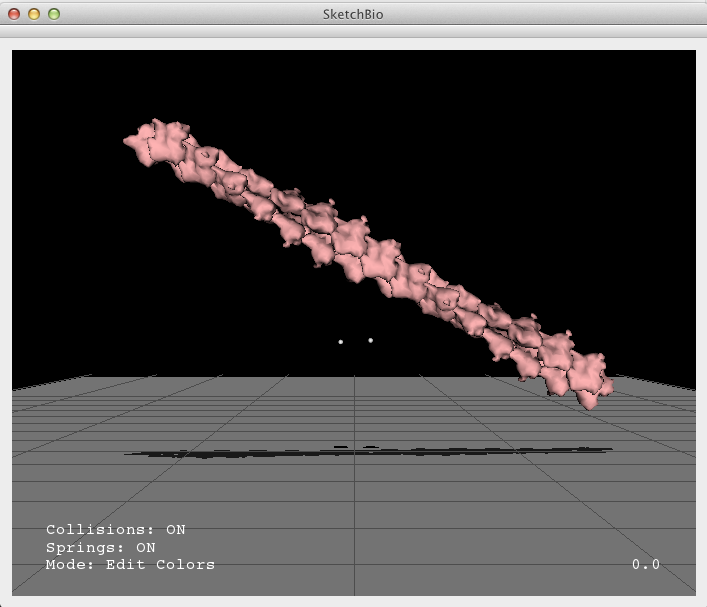
\includegraphics[width=0.8\columnwidth]{crystal_actin.png}
\caption{A screenshot from SketchBio showing an actin filament created with the crystal-by-example function and using the transformation matrix from the PDB data from one monomer to the next.}
\label{fig:crystal_actin}
\end{figure}

\paragraph*{Grouping:}
Grouping of molecules into larger units is also supported to make constructing larger order structures easier.  This also allows smooth animation of objects that are moving together without the small variations that even the most careful hand-placement will create.  Copy and paste is also implemented and both single objects and groups can be copied and pasted, even between sessions.

\paragraph*{Connectors:}
SketchBio also has connectors that can be added between objects.  These can act like springs and apply forces to keep objects positioned relative to each other or they can simply indicate that two objects are connected.  For many proteins there are regions for which the structure is unknown and these regions can be represented with these connectors.  As it is not the intent that SketchBio simulate accurate forces on the molecules it displays, only very simple physics is applied and an extremely viscous fluid is assumed which negates all momentum.

\subsection*{Pose Mode and Collision Detection}
An observation about the motions of objects in SketchBio is: for most of the time working with the program, the only objects that move are those directly being manipulated by the user.  The user may even find it annoying if the object they are moving pushes the object they are attempting to dock it with away every time they accidentally collide.  Therefore one simplification that can be made to collision detection is to employ what we call pose mode physics.  In pose mode physics, only the objects directly manipulated by the user are allowed to move.  Each other object is fixed in place and does not even move due to collision response forces.  This allows an easier time docking the molecules as the molecule not being held does not get pushed away while also allowing the collision tests between the objects that the user is not interacting with to be skipped since it is known that these objects did not move.  The only way that those objects could be in collision was if they were already in collision before.  If the collision response failed to fix the collision then, it will not fix it now, so their tests can be skipped.  This means that only collisions involving the objects that the user is moving need to be checked.  This reduces the number of collision tests to $m*n$ where m is the number of objects that the user is currently moving.  The typical number of objects that the user moves at a time is 1 or a small constant in the case of moving a group, which reduces the number of collision tests needed to $\mathcal{O}(n)$ in this expected case.

\subsection*{Crystal-by-example Collision Detection}
There are two ways that the user can interact with a crystal-by-example structure: moving the entire structure as a unit, or adjusting the internal transformation to change the shape of the structure.  In the first case, only collision tests between the structure and the other objects in the scene need to be done, and the above bound applies to the number of tests  Since the structure was moved as a unit, its internal geometry did not change and if there were no internal collisions to begin with, there will be none after it was moved.  In the second case, the internal structure did change and both internal and external collisions must be tested.  External collisions must test every object in the structure with every external object as above.  Let $X_i$ be the ith object in the crystal by example structure with $X_0$ and $X_1$ being the two base object in the structure.  Let $T_{i,j}$ be the transformation matrix from $X_i$ to $X_j$.  The definition of the crystal-by-example structure is that $T_{i,i+1}$ is the same for all $i$ and the geometries of all the $X_i$s are the same.  Since the geometries and transformations are the same, if there is a collision between the $ith$ and $(i+1)th$ objects anywhere in the structure, then there is also a collision between the $0th$ and $1st$ objects.  Thus testing only this one pair performs the work of n-1 tests where n is the number of objects in the structure.  This same argument holds for any $i$ and $i+k$, the $0th$ and $kth$ objects have the same relative positions and the same collisions.  Thus only the $0th$ object in the structure needs to be tested against the others which allows $\mathcal{O}(n)$ tests to suffice for all internal collisions in a repetitive structure of $n$ elements.

% a possible alternate talking about shadow technique XXX - Russ look at this please.
%\subsection*{Drop Shadows}
%Initial testing of the application revealed that determining the relative depth between an object and the user's hand or between two objects was the most difficult part of using SketchBio.  Since the budget constraints of our potential users prevented the use of stereo displays and head tracking, the next best techniques according to Hendrix are drop lines from the centers of objects and shadows \cite{Hendrix1995103}.  Drop lines give the best information about absolute positions of objects while shadows give better information about distances between objects since the radius of the object must still be estimated using drop lines.  Combining these two ideas, SketchBio uses drop shadows, the geometry of the object projected onto a plane below the camera.  The result is similar to shadows with a light source at infinity and gives both absolute position information but also relative depth between objects.

%\begin{figure*}[t!]
%  \centering
%  \includegraphics[height=3.5in]{placeholder.eps}
%  \caption{Example two-column figure. To insert a single column figure, remove the * in the two figure tags. }
%  \label{fig:interface}
%\end{figure*}

\subsection*{Success Measures}

XXX - write this

\section*{Results}
\subsection*{Model Creation}

\begin{figure}[h]
\centering
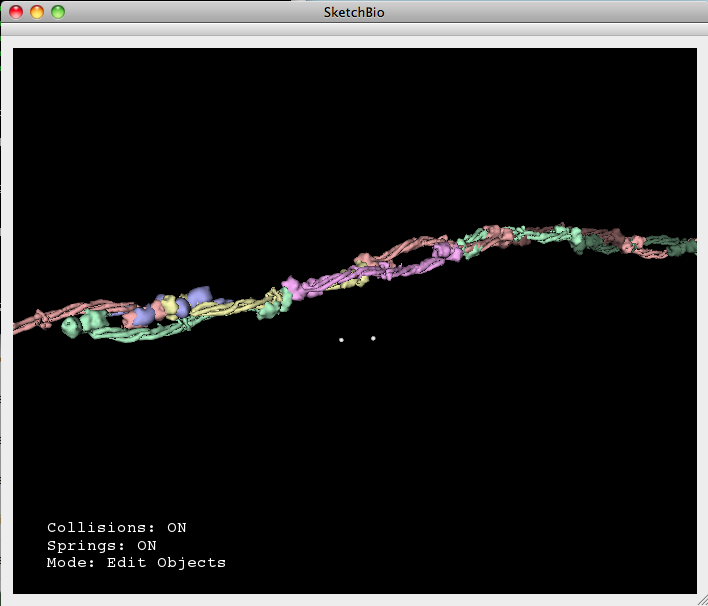
\includegraphics[width=0.8\columnwidth]{joe_test.png}
\caption{A view of the model Joe Hsiao created with SketchBio to compare usibility with UCSF Chimera}
\label{fig:joe_test}
\end{figure}

Constructing the protofibril models for Susan Lord took Resource computer scientist Joe Hsiao 3-3.5 hours by hand-editing transformations within Chimera (a task challenging to teach to biologists).  Using an early prototype of SketchBio, he constructed the protofibril seen in Figure \ref{fig:joe_test} in 1.5 hours (a task we'd expect a collaborator to do just as rapidly).  From this demonstration the lack of depth cues became apparent and later the shadow plane was added.  This should reduce the amount of time needed to construct the protofibril model in SketchBio even further.  XXX - get new time for Joe

\begin{figure}[h]
\centering
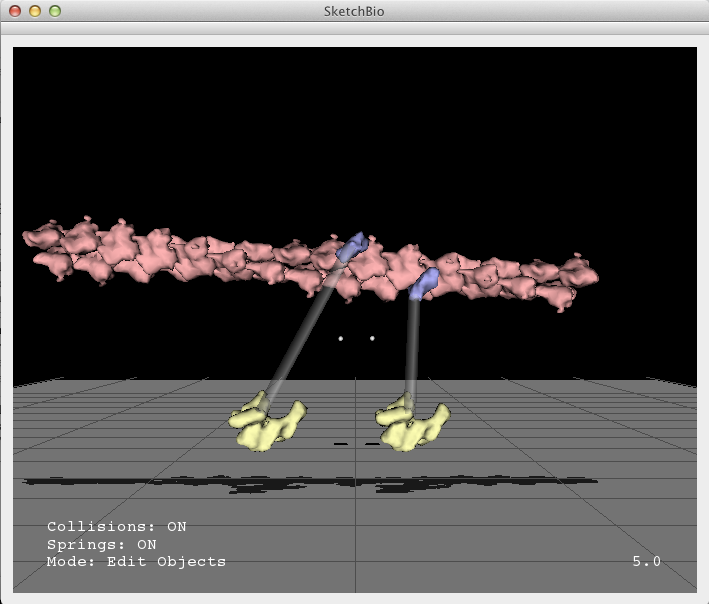
\includegraphics[width=0.8\columnwidth]{peter_model.png}
\caption{A scene from a video created by Peter Thompson in SketchBio.  Approximately the same timestep is shown rendered at its full resolution in Figure \ref{fig:peter_video}}
\label{fig:peter_model}
\end{figure}


Collaborator Peter Thompson, a biochemisty graduate student, created an animation of vinculin binding to an actin fiber.  The animation is based on the model presented in a recent paper.  He was able to create the video with minimal help from a computer scientist and plans to use it in an upcoming talk.  The model in SketchBio is shown in Figure \ref{fig:peter_model} and a frame from the resulting video at approximately the same time is shown in Figure \ref{fig:peter_video}.  Peter has said that to make a single animation, he would use Powerpoint animations to create a lower quality animation more quickly, but for making more than one animation, he thinks it is worth it to learn SketchBio.


\begin{figure}[h!]
\centering
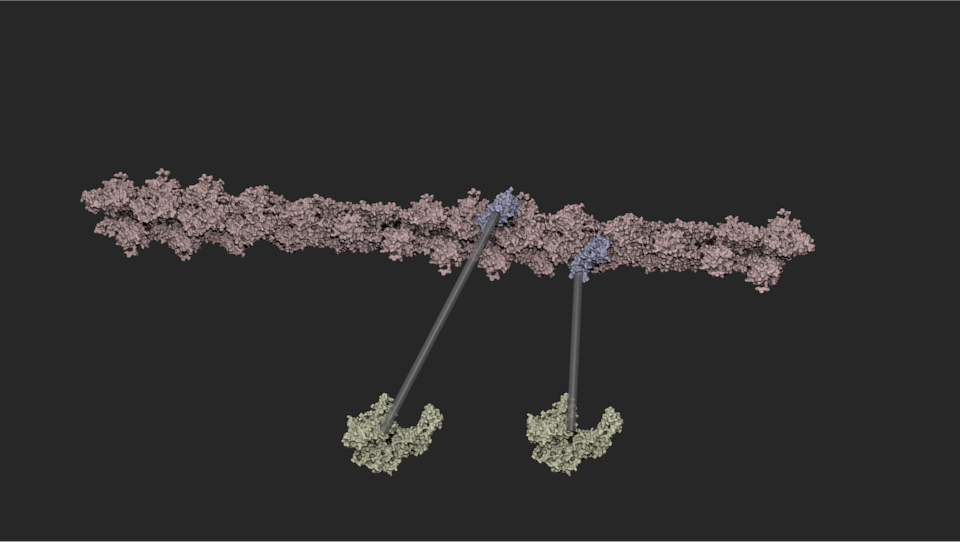
\includegraphics[width=0.8\columnwidth]{peter_video.png}
\caption{A frame from the video created by Peter Thompson.  This shows the tail domains of vinculin binding to an actin filament and slowing its motion.  This video was created in SketchBio as seen in Figure \ref{fig:peter_model} and rendered via the export to Blender feature.}
\label{fig:peter_video}
\end{figure}

% XXX - talk about the reuse instead of reimplementation goal

\subsection*{Collision Detection Speed-ups}

\section*{Discussion}

\section*{Conclusions} % XXX - rewrite this
The current state of SketchBio allows users to position molecules with collision detection, create repeated structures with crystal-by-example, and create animations by placing keyframes in time to specify the paths the objects take.  It has already been used by a scientist to create a video that he feels is usable in a presentation to others in his field.  This animation was based on a model from a paper he had read and wished to present.  He also created a model based on a second paper using the charge-colored surfaces to see the interaction propsed.  The developers of the tool were able to create an animation showing an approximation of the interaction between several of the molecules in about 30 minutes.  Although more work is required, this use shows that this tool is capable of letting scientists create models and animations without directly including a computer scientist or animator in the process.

\subsection*{Acknowledgements}
This work was supported by NIH grant 5-P41-EB002025.

Molecular graphics and analyses were performed with the UCSF Chimera package. Chimera is developed by the Resource for Biocomputing, Visualization, and Informatics at the University of California, San Francisco (supported by NIGMS P41-GM103311).

%%%%%%%%%%%%%%%%%%%%%%%%%%%%%%%%%%%%%%%%%%%%%% 
%%                                          %%
%% Backmatter begins here                   %%
%%                                          %%
%%%%%%%%%%%%%%%%%%%%%%%%%%%%%%%%%%%%%%%%%%%%%%

\begin{backmatter}

\section*{List of abbreviations used}
PQP: \textit{Proximity Query Package}, VRPN: \textit{Virtual Reality Peripheral Network}, PDB: \textit{protein data bank}.

\section*{Competing interests}
The authors declare that they have no competing interests.


%%%%%%%%%%%%%%%%%%%%%%%%%%%%%%%%%%%%%%%%%%%%%%%%%%%%%%%%%%%%%
%%                  The Bibliography                       %%
%%                                                         %%
%%  Bmc_mathpys.bst  will be used to                       %%
%%  create a .BBL file for submission.                     %%
%%  After submission of the .TEX file,                     %%
%%  you will be prompted to submit your .BBL file.         %%
%%                                                         %%
%%                                                         %%
%%  Note that the displayed Bibliography will not          %%
%%  necessarily be rendered by Latex exactly as specified  %%
%%  in the online Instructions for Authors.                %%
%%                                                         %%
%%%%%%%%%%%%%%%%%%%%%%%%%%%%%%%%%%%%%%%%%%%%%%%%%%%%%%%%%%%%%

% if your bibliography is in bibtex format, use those commands:
\bibliographystyle{bmc-mathphys} % Style BST file
\bibliography{sources}      % Bibliography file (usually '*.bib' )

% or include bibliography directly:
% \begin{thebibliography}
% \bibitem{b1}
% \end{thebibliography}

%%%%%%%%%%%%%%%%%%%%%%%%%%%%%%%%%%%
%%                               %%
%% Figures                       %%
%%                               %%
%% NB: this is for captions and  %%
%% Titles. All graphics must be  %%
%% submitted separately and NOT  %%
%% included in the Tex document  %%
%%                               %%
%%%%%%%%%%%%%%%%%%%%%%%%%%%%%%%%%%%

%%
%% Do not use \listoffigures as most will included as separate files

%\section*{Figures}
%  \begin{figure}[h!]
 % \caption{\csentence{Sample figure title.}
  %    A short description of the figure content
   %   should go here.}
   %   \end{figure}

%\begin{figure}[h!]
 % \caption{\csentence{Sample figure title.}
  %    Figure legend text.}
  %    \end{figure}

%%%%%%%%%%%%%%%%%%%%%%%%%%%%%%%%%%%
%%                               %%
%% Tables                        %%
%%                               %%
%%%%%%%%%%%%%%%%%%%%%%%%%%%%%%%%%%%

%% Use of \listoftables is discouraged.
%%
%\section*{Tables}
%\begin{table}[h!]
%\caption{Sample table title. This is where the description of the table should go.}
 %     \begin{tabular}{cccc}
%        \hline
 %          & B1  &B2   & B3\\ \hline
 %       A1 & 0.1 & 0.2 & 0.3\\
 %       A2 & ... & ..  & .\\
 %       A3 & ..  & .   & .\\ \hline
 %     \end{tabular}
%\end{table}

%%%%%%%%%%%%%%%%%%%%%%%%%%%%%%%%%%%
%%                               %%
%% Additional Files              %%
%%                               %%
%%%%%%%%%%%%%%%%%%%%%%%%%%%%%%%%%%%

%\section*{Additional Files}
%  \subsection*{Additional file 1 --- Sample additional file title}
%    Additional file descriptions text (including details of how to
%    view the file, if it is in a non-standard format or the file extension).  This might
%    refer to a multi-page table or a figure.

%  \subsection*{Additional file 2 --- Sample additional file title}
%    Additional file descriptions text.

\end{backmatter}
\end{document}
